% Copyright (C) 2012 Shi.Zhan <g.shizhan.g@gmail.com>
%
% Permission is hereby granted, free of charge, to any person obtaining a copy of this software and associated documentation files (the "Software"), to deal in the Software without restriction, including without limitation the rights to use, copy, modify, merge, publish, distribute, sublicense, and/or sell copies of the Software, and to permit persons to whom the Software is furnished to do so, subject to the following conditions:
%
% The above copyright notice and this permission notice shall be included in all copies or substantial portions of the Software.
%
% THE SOFTWARE IS PROVIDED "AS IS", WITHOUT WARRANTY OF ANY KIND, EXPRESS OR IMPLIED, INCLUDING BUT NOT LIMITED TO THE WARRANTIES OF MERCHANTABILITY, FITNESS FOR A PARTICULAR PURPOSE AND NONINFRINGEMENT. IN NO EVENT SHALL THE AUTHORS OR COPYRIGHT HOLDERS BE LIABLE FOR ANY CLAIM, DAMAGES OR OTHER LIABILITY, WHETHER IN AN ACTION OF CONTRACT, TORT OR OTHERWISE, ARISING FROM, OUT OF OR IN CONNECTION WITH THE SOFTWARE OR THE USE OR OTHER DEALINGS IN THE SOFTWARE.
%
% 课程:人机交互技术及应用
% 班级:传播学1001班
% 课时:40学时,2012年秋季1~10周,每周一、三
% 地点:东九楼D212
% 主页:http://code.google.com/p/hci-course/
% 教师:施展 
% 单位:华中科技大学 武汉光电国家实验室
%
\documentclass{beamer}
\usepackage{fontspec,xunicode,xltxtra,beamerthemesplit}
%\usetheme{Hannover} % White background
\usetheme{Berkeley} % Blue background
\setmainfont[
	BoldFont={WenQuanYi Zen Hei},
	ItalicFont={WenQuanYi Micro Hei}
]{WenQuanYi Micro Hei}
\setsansfont[
	BoldFont={WenQuanYi Zen Hei},
	ItalicFont={WenQuanYi Micro Hei}
]{WenQuanYi Micro Hei}

% 中文环境自动换行
\XeTeXlinebreaklocale "zh"
\XeTeXlinebreakskip = 0pt plus 1pt

% 中文环境修正导航栏
\makeatletter
\def\beamer@linkspace#1{
	\begin{pgfpicture}{0pt}{-1.5pt}{#1}{5.5pt}
		\pgfsetfillopacity{0}
		\pgftext[x=0pt,y=-1.5pt]{.}
		\pgftext[x=#1,y=5.5pt]{.}
	\end{pgfpicture}
}
\makeatother

% diagrams
\usepackage{tikz}
\usetikzlibrary{arrows,shapes}

% full page image
\newcommand{\fullPageImage}[2]{
	{
		\usebackgroundtemplate{\includegraphics[width=\paperwidth, height=\paperheight]{#1}}
		\frame[plain]{#2}
	}
}

\title{人机交互技术}
\author{施展}
\institute{华中科技大学~武汉光电国家实验室}
\date{\today}
\titlegraphic{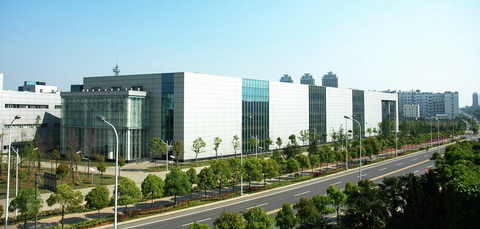
\includegraphics[width=2cm]{images/wnlo.jpg}}

\begin{document}

\begin{frame}
	\titlepage
\end{frame}

\begin{frame}
	\frametitle{内容提要}
	\tableofcontents
\end{frame}

\section{第七讲}
\begin{frame}
	\frametitle{第七讲 Web界面设计}
	\begin{itemize}
		\item 熟悉Web设计的原则及Web界面设计包含的元素。
		\item 掌握主要Web界面设计语言和技术,并灵活应用。
		% adjust to html5, introduce the most recent and promising techonology
	\end{itemize}
\end{frame}

\subsection{Web界面及相关概念}
\begin{frame}
	\frametitle{Web界面及相关概念}
	\beamertemplatetransparentcovereddynamicmedium
	\begin{itemize}[<+->]
		\item 万维网 World Wide Web, WWW
		\begin{itemize}
			\item 由高能核物理学家Tim Berners-Lee建立雏形:
			\begin{itemize}
				\item 一个能够整合各种资源、文件及多媒体的系统,让使用者方便地取得不同媒体的资料。
			\end{itemize}
			\item 建立在客户/服务器模型之上
			\begin{itemize}
				\item 超文本标记语言 Hypertext Markup Language, HTML~\cite{berners1995hypertext}
				\item 超文本传输协议 Hypertext Transport Protocols, HTTP~\cite{fielding1999hypertext}
				\item 通过Internet把遍布世界各地的服务器连接起来,提供各种服务,具有一致用户界面的信息浏览功能。
			\end{itemize}
		\end{itemize}
	\end{itemize}
\end{frame}

\begin{frame}
	\frametitle{超文本与超媒体}
	\begin{center}
	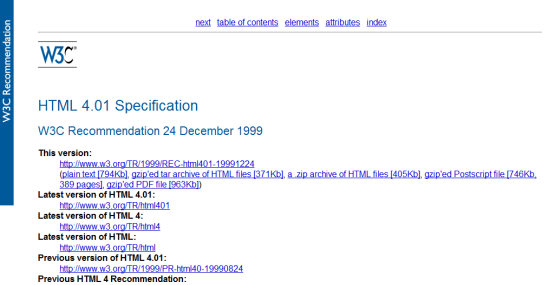
\includegraphics[width=.8\textwidth]{images/html-specs.png}
	\end{center}
\end{frame}

\begin{frame}
	\frametitle{超文本与超媒体}
	\beamertemplatetransparentcovereddynamicmedium
	\begin{itemize}
		\pause
		\item 超文本 Hypertext
		\begin{itemize}
			\item 是一种使用于文本、图形或其他信息的组织形式,非线性的信息组织。
			\item 使得单一的信息元素之间可以相互交叉引用,这种引用并不是通过复制来实现的,而是通过指向对方的地址字符串来指引用户获取相应的信息。 
		\end{itemize}
		\pause
		\item 超媒体 Hypermedia
		\begin{itemize}
			\item 利用超文本形式组织起来的文件不仅仅是文本,也可以是图、文、声、像以及视频等多媒体形式的文件。
			\item 这些多媒体信息就构成了所谓的超媒体 。
		\end{itemize}
	\end{itemize}
\end{frame}

% http://edward.oconnor.cx/2009/05/what-the-web-platform-is-not
\fullPageImage{images/w3-stack.png}{
	\pause
	\begin{beamerboxesrounded}[shadow=true]{W3C的展望}
	The Web stack envisioned by the W3C in 2004
	\end{beamerboxesrounded}
}

% http://www.concinnity.dk/wp-content/uploads/2010/09/Nova-Spivack1.jpg
\fullPageImage{images/nova-spivack1.jpg}{
	\pause
	\begin{beamerboxesrounded}[shadow=true]{华丽的现实}
	各种媒体内容、技术、语言林立 \dots
	\end{beamerboxesrounded}
}

\begin{frame}
	\frametitle{Web的发展趋势}
	\beamertemplatetransparentcovereddynamicmedium
	\begin{itemize}
		\item Web的爆炸性发展
		\begin{itemize}
			\item 各种媒体
			\item 各类交互
			\item 广泛渗透 
		\end{itemize}
		\pause
		\item 信息交换 \& W3C标准: XML
		\pause
		\item 交互方式 \& Web 2.0 \& 云 \& 对桌面应用的挑战
		\pause
		\item 知识与理解 \& Web 3.0 \& Semantic Web
	\end{itemize}
\end{frame}

\begin{frame}
	\frametitle{Web的发展趋势}
	\begin{itemize}
		\item 展望语义网 Semantic Web
	\end{itemize}
	\begin{center}
	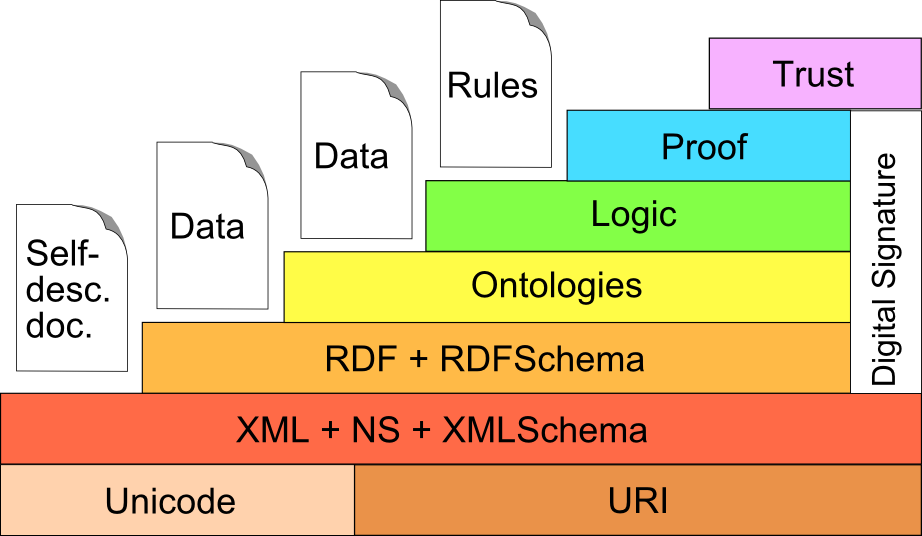
\includegraphics[width=.8\textwidth]{images/semantic-web-stack.png}
	\end{center}
\end{frame}

\begin{frame}
	\frametitle{Web界面设计问题的提出}
	\beamertemplatetransparentcovereddynamicmedium
	\begin{itemize}
		\item 问题表现:
		\begin{itemize}
			\item 外在原因: 外观是否友好直观,富有吸引力。
			\item 内在原因: 响应是否及时准确,具备扩张力。
		\end{itemize}
		\pause
		\item 问题核心: 
		\begin{itemize}
			\item 人性化的设计: 如何根据人的心理、生理特征,运用技术手段,创造简单、友好的界面。
		\end{itemize}
	\end{itemize}
\end{frame}

\subsection{Web界面设计原则}
\begin{frame}
	\frametitle{Web界面设计原则}
	% http://www.w3.org/DesignIssues/
	\beamertemplatetransparentcovereddynamicmedium
	\begin{enumerate}[<+->]
		\item 以用户为中心
		\item 一致性
		\item 简洁与明确
		\item 体现特色
		\item 兼顾不同的浏览器
		\item 明确的导航设计
	\end{enumerate}
\end{frame}

\begin{frame}
	\frametitle{Web界面设计原则~{\small 以用户为中心}}
	\beamertemplatetransparentcovereddynamicmedium
	\begin{itemize}[<+->]
		\item 网站是给什么人用的?
		\item 关于腾讯QQ与TM、开心网和人人网
	\end{itemize}
\end{frame}

\begin{frame}
	\frametitle{Web界面设计原则~{\small 一致性}}
	\beamertemplatetransparentcovereddynamicmedium
	\begin{itemize}
		\item 内容一致:
		\begin{itemize}
			\item Web网站显示的信息、数据整齐规范 \dots
		\end{itemize}
		\pause
		\item 形式一致:
		\begin{itemize}
			\item Web界面设计的版式、构图、布局、色彩以及它们所呈现出的风格特点
		\end{itemize}
		\pause
		\item www.hust.edu.cn
	\end{itemize}
\end{frame}

\begin{frame}
	\frametitle{Web界面设计原则~{\small 简洁与明确}}
	% http://en.wikipedia.org/wiki/KISS_principle
	\beamertemplatetransparentcovereddynamicmedium
	\begin{center}
	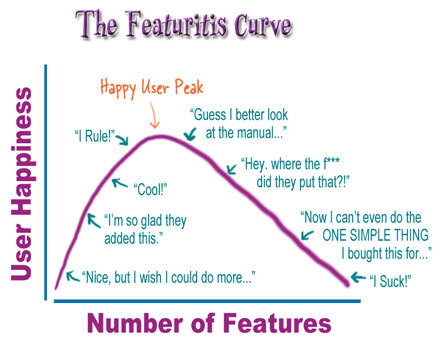
\includegraphics[width=.5\textwidth]{images/featuritis-2.jpg}
	\end{center}
	\pause
	\begin{itemize}[<+->]
		\item "Keep it simple, stupid!"\\
		{\tiny The acronym was coined by Kelly Johnson, lead engineer at the Lockheed Skunk Works (creators of the Lockheed U-2 and SR-71 Blackbird spy planes, among many others).}
	\end{itemize}
\end{frame}

\begin{frame}
	\frametitle{Web界面设计原则~{\small 简洁与明确}}
	% http://www.zhangping.name/2010/08/14/pm-keep-it-simple-stupid/
	\beamertemplatetransparentcovereddynamicmedium
	\begin{itemize}
		\item 关于 Windows 自身的挑战 \dots
		\pause
		\item 关于Web应用
		\begin{itemize}
			\item Google: \uncover<3->{搜索你想要的}
			\item Facebook: \uncover<4->{和你的朋友保持联系}
			\item Twitter: \uncover<5->{说说你在做什么}
			\item FourSquare: \uncover<6->{报告你现在的位置}
		\end{itemize}
		\uncover<7->{\item GMail 与 Labs 以及追随者们 \dots}
		% Gmail在对Lab上的处理可能是个很好的例子,与其面向所有用户推出新功能,Gmail把Lab作为新功能的可选项,这样当用户不喜欢Lab的时候,可以轻易地关掉它。
	\end{itemize}
\end{frame}

\begin{frame}
	\frametitle{Web界面设计原则~{\small 体现特色}}
	\beamertemplatetransparentcovereddynamicmedium
	\begin{itemize}
		\item 清楚地了解Web网站背景、体现主题和服务对象的基本情况,选择合适的表现手法,展示关键信息和特色内容,并形成独特、鲜明的风格。
		\pause
		\item http://mole.61.com/
		% 专为中国7-12岁儿童设计的安全健康益智的虚拟互动社区,每个儿童化身可爱的小鼹鼠摩尔,成为这个虚拟世界的主人,社区融合虚拟形象 ...
	\end{itemize}
\end{frame}

\begin{frame}
	\frametitle{Web界面设计原则~{\small 兼顾不同的浏览器}}
	\beamertemplatetransparentcovereddynamicmedium
	\begin{itemize}
		\item 不同浏览器类别和版本在功能支持上有所区别
		\pause
		\item 关于IE6的“老大难”
	\end{itemize}
\end{frame}

\begin{frame}
	\frametitle{Web界面设计原则~{\small 明确的导航设计}}
	\beamertemplatetransparentcovereddynamicmedium
	\begin{itemize}[<+->]
		\item F布局
	\end{itemize}
\end{frame}

% http://webdesign.tutsplus.com/articles/design-theory/understanding-the-f-layout-in-web-design/
\fullPageImage{images/heatmap.jpg}{}
\fullPageImage{images/f-wireframe.jpg}{}
\fullPageImage{images/f-pattern-2.jpg}{}

\subsection{Web界面要素设计}
\begin{frame}
	\frametitle{Web界面要素设计}
	\beamertemplatetransparentcovereddynamicmedium
	\begin{enumerate}[<+->]
		\item Web界面规划
		\item 文化与语言
		\item 内容、风格与布局、色彩设计
		\item 文本设计
		\item 多媒体元素设计
	\end{enumerate}
\end{frame}

\begin{frame}
	\frametitle{Web界面要素设计~{\small Web界面规划}}
	\beamertemplatetransparentcovereddynamicmedium
	\begin{itemize}[<+->]
		\item .
	\end{itemize}
\end{frame}

\begin{frame}
	\frametitle{Web界面要素设计~{\small 文化与语言}}
	\beamertemplatetransparentcovereddynamicmedium
	\begin{itemize}[<+->]
		\item .
	\end{itemize}
\end{frame}

\begin{frame}
	\frametitle{Web界面要素设计~{\small 内容、风格与布局、色彩设计}}
	\beamertemplatetransparentcovereddynamicmedium
	\begin{itemize}[<+->]
		\item .
	\end{itemize}
\end{frame}

\begin{frame}
	\frametitle{Web界面要素设计~{\small 文本设计}}
	\beamertemplatetransparentcovereddynamicmedium
	\begin{itemize}[<+->]
		\item .
	\end{itemize}
\end{frame}

\begin{frame}
	\frametitle{Web界面要素设计~{\small 多媒体元素设计}}
	\beamertemplatetransparentcovereddynamicmedium
	\begin{itemize}[<+->]
		\item .
	\end{itemize}
\end{frame}

\subsection{Web界面基本技术}
% http://sixrevisions.com/web-technology/web-languages-decoded/
\fullPageImage{images/abbreviation-overload.png}{}

\begin{frame}
	\frametitle{Web界面基本设计技术}
	\beamertemplatetransparentcovereddynamicmedium
	\begin{itemize}[<+->]
		\item 超文本标记语言 HTML
		\item 富英特网应用 Rich Internet Application 
		\item 客户端脚本语言 JavaScript 
		\item 服务器端脚本语言 Dynamic Web Page
	\end{itemize}
\end{frame}

\begin{frame}
	\frametitle{Web界面基本技术~{\small HTML}}
	\beamertemplatetransparentcovereddynamicmedium
	\begin{itemize}[<+->]
		\item .
	\end{itemize}
\end{frame}

\begin{frame}
	\frametitle{Web界面基本技术~{\small RIA}}
	\beamertemplatetransparentcovereddynamicmedium
	\begin{itemize}[<+->]
		\item JavaApplet, Flash, Silverlight
		\item 平台兼容、平台锁定?
		\item HTML 5 canvas \dots
	\end{itemize}
\end{frame}

\begin{frame}
	\frametitle{Web界面基本技术~{\small JavaScript}}
	\beamertemplatetransparentcovereddynamicmedium
	\begin{itemize}[<+->]
		\item 客户端
		\item 服务器端
	\end{itemize}
\end{frame}

\begin{frame}
	\frametitle{Web界面基本技术~{\small Dynamic Web Page}}
	\beamertemplatetransparentcovereddynamicmedium
	\begin{itemize}[<+->]
		\item 公用网关接口 Common Gateway Interface, CGI
		\begin{itemize}
			\item 早期可使用普通高级语言编写CGI程序以处理特定服务器端信息
			\begin{itemize}
				\item 如 Visual Basic, Delphi 或 C/C++ \dots
			\end{itemize}
			\item 编程困难、效率低下、修改复杂
			\item CGI改进
			\begin{itemize}
				\item FastCGI
				\item WSGI
			\end{itemize}
		\end{itemize}
	\end{itemize}
\end{frame}

\begin{frame}
	\frametitle{Web界面基本技术~{\small Dynamic Web Page}}
	% http://en.wikipedia.org/wiki/Dynamic_web_page
	\begin{center}
	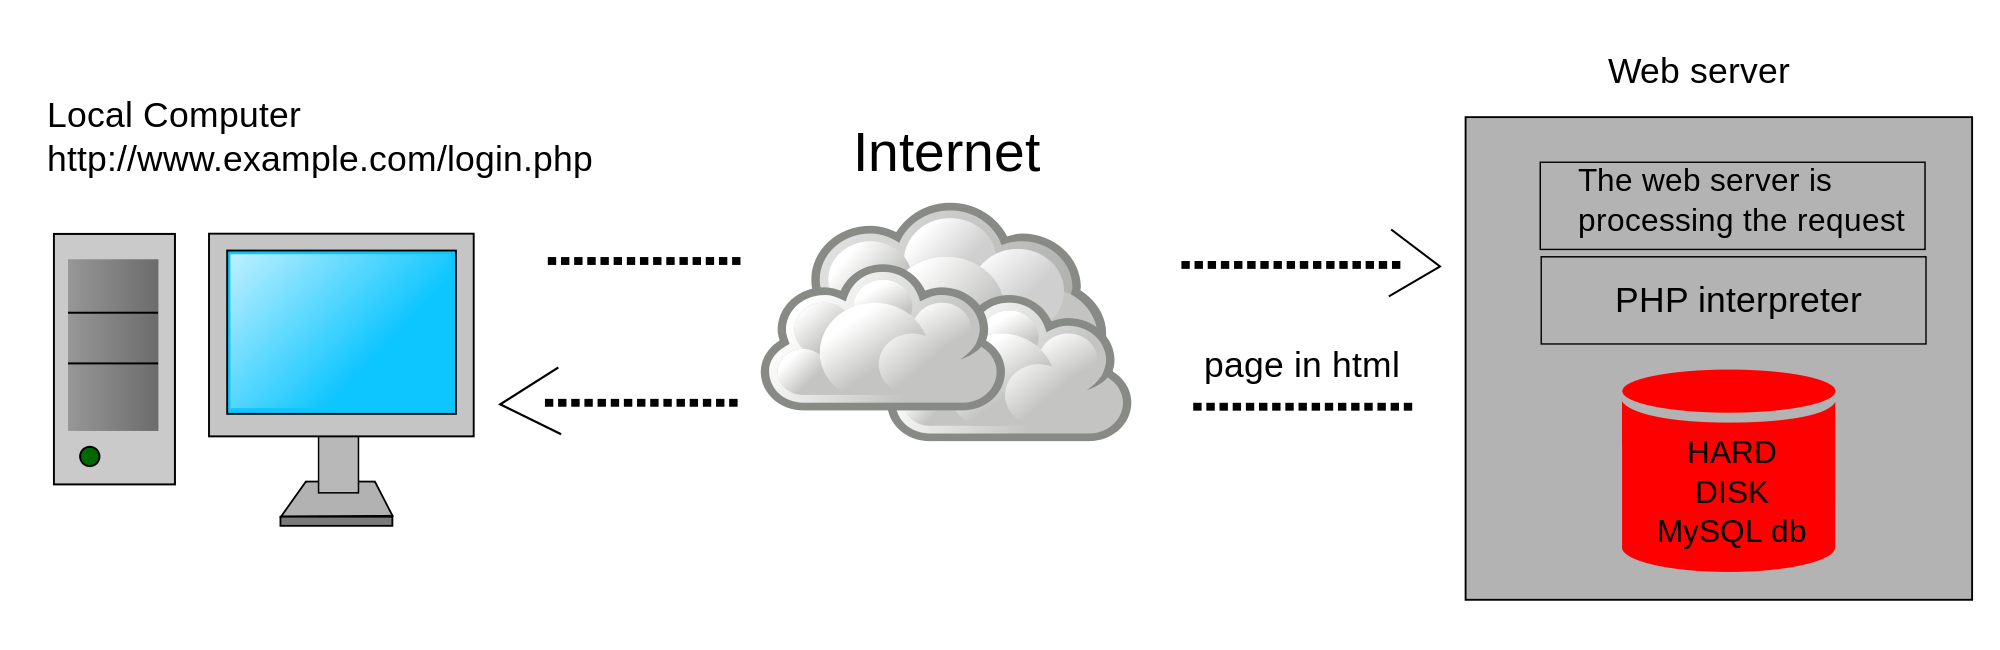
\includegraphics[width=.8\textwidth]{images/2000px-Scheme_dynamic_page_en.svg.png}
	\end{center}
	\beamertemplatetransparentcovereddynamicmedium
	\begin{itemize}[<+->]
		\item 动态页面语言
		\begin{itemize}
			\item ASP/ASPX, JSP, PHP, Perl, Python, Ruby \dots
			\begin{itemize}
				\item 与数据库交互以更新页面内容
				\item 处理HTML表单与URL参数
			\end{itemize}
		\end{itemize}
	\end{itemize}
\end{frame}

\begin{frame}
	\frametitle{Web界面基本技术~{\small AJAX}}
	\beamertemplatetransparentcovereddynamicmedium
	\begin{itemize}[<+->]
		\item 将客户端脚本与服务器端脚本组合起来,提高交互实时性、丰富其内容
		\item Asynchronous JavaScript and XML - AJAX
	\end{itemize}
\end{frame}

\subsection{Web界面新进展}
\begin{frame}
	\frametitle{Web界面新进展——HTML5}
	% http://www.w3school.com.cn/html5/html_5_intro.asp
	\beamertemplatetransparentcovereddynamicmedium
	\begin{itemize}
		\item HTML5 是 W3C 与 WHATWG 合作的结果。~\cite{hickson2007html}
		\item WHATWG 致力于 web 表单和应用程序,而 W3C 专注于 XHTML 2.0。
		\item 在 2006 年,双方决定进行合作,来创建一个新版本的 HTML。
		\pause
		\item 为 HTML5 建立的一些规则:
		\begin{itemize}
			\item 新特性应该基于 HTML、CSS、DOM 以及 JavaScript。
			\item 减少对外部插件的需求(比如 Flash)
			\item 更优秀的错误处理
			\item 更多取代脚本的标记
			\item HTML5 应该独立于设备
			\item 开发进程应对公众透明
		\end{itemize}
	\end{itemize}
\end{frame}

\begin{frame}
	\frametitle{Web界面基本技术~{\small HTML 5}}
	\beamertemplatetransparentcovereddynamicmedium
	\begin{columns}
	\column{.5\textwidth}
	\begin{itemize}[<+->]
		\item HTML5 中的一些有趣的新特性:
		\begin{itemize}
			\item {\tiny 用于绘画的 canvas 元素}
			\item {\tiny 用于媒介回放的 video 和 audio 元素}
			\item {\tiny 对本地离线存储的更好的支持}
			\item {\tiny 新的特殊内容元素: article、footer、header、nav、section}
			\item {\tiny 新的表单控件: calendar、date、time、email、url、search}
		\end{itemize}
	\end{itemize}
	\column{.5\textwidth}
	
\includegraphics[width=0.9\textwidth]{images/html-5.png}
	\end{columns}
\end{frame}

\section{小结}
\begin{frame}
	\frametitle{小结}
	\begin{itemize}
		\item 了解、认识Web界面及相关概念与关键技术
		\item 探讨Web界面设计原则、基本要素
	\end{itemize}
\end{frame}

\begin{frame}
	\frametitle{参考文献}
	\bibliographystyle{plain}
	\bibliography{hci}
\end{frame}

\end{document}